\section{Introduction}

In the context of natural phenomena modelling, verification refers to the process of confirming that the final program’s output mathematically corresponds to the analytically derived, expected outcome. Validation refers to the process of confirming that the model can, to some degree of accuracy, model the real phenomena it is meant to predict. In simplified terms, verification tests simplified cases that can be modelled both computationally and analytically, and compares the results. Validation tests real world, complex cases that can only be studied computationally and historically. These two processes give greater confidence (but not guarantee) that the model is performing as it is expected, and can reliably predict future events. 

ASTM E1355 Standard Guide for Evaluating the Predictive Capability of Deterministic Fire Models (2018) defines model verification as “the process of determining that the implementation of a calculation method accurately represents the developer’s conceptual description of the calculation method and solution to the calculation method.” Slightly different definitions of model verification are used by other standards in other industries, but in general verification involves assessing whether the underlying mathematical formulation is correctly implemented in the source code - or “is the math right”. ASTM E1355 Standard Guide for Evaluating the Predictive Capability of Deterministic Fire Models (2018) defines model validation as “the process of determining the degree to which a calculation method is an accurate representation of the real-world from the perspective of the intended uses of the calculation method.”

Verification and validation of wildfire spread models has its own intricacies and particularities, as the range of methodologies that can be employed to model wildfire spread are broad and varied. Sullivan categorises the plethora of models in the literature as spanning a spectrum between empirical (purely relying on experimental correlations and interpolations) and physical (purely relying on conservation laws and heat and mass transfer laws). Most wildfire models are somewhere inbetween, with some degree of physical reasoning and calibration required by all models. ELMFIRE would be classified as a semi-empirical model, as it primarily uses physically-derived equation with empirical, experiment-driven parameterization. 

Model verification is typically approached by simulating simple canonical problems and comparing model outputs to exact solutions, where available. ELMFIRE has been subjected to extensive model verification exercises since development began in 2010. In an effort to promote transparency and authenticity, ELMFIRE’s mathematical formulation is documented in the Technical Reference, its source code is maintained in a public Git repository, and several model verification test cases.

This guide will present the results of a verification and validation study of ELMFIRE. A series of simplified cases will first be presented, with quantitative and qualitative comparison of the computational and analytical results. Following that, a series of historical wildfires will be modelled in ELMFIRE. The results will be compared to establish ELMFIRE's ability to work on real, complex landscapes. 

\section{Verification Test Cases}

The verification of ELMFIRE will be based on the WUI-NITY project verification guide (WUI-NITY 2), where a wildfire spread model verification method is described, and later applied in a benchmarking study. The verification test suggests small landscapes with five simplified scenarios:
\begin{itemize}
 \item \textbf{``Point''}: Uniform fuel, flat landscape, zero wind, ignition at the center of the landscape.
 \item \textbf{``Windy''}: Uniform fuel, flat landscape, northern wind, ignition at the north part of the landscape.
 \item \textbf{``Valley''}: Uniform fuel, a shallow landscape rise to the east and a steep rise to the west, zero wind, ignition at the center of the landscape.
 \item \textbf{``Fuel Quadrant''}: Different fuels at each quadrant of the landscape, flat landscape, zero wind, ignition at the center of the landscape.
 \item \textbf{``Complex''}: (an amalgamation of the previous cases) Different fuels at each quadrant of the landscape, a shallow landscape rise to the east and a steep rise to the west, northern wind, ignition at the center. 
\end{itemize}

Each of these tests verifies the model against a separate parameter, with the final one superimposing the previous cases to test their interaction. For this verification guide, additional tests are proposed to expand the parameters being examined and verified. These extra tests follow from the submodel breakdown identified in the main guide. 

\begin{itemize}
 \item \textbf{``Moisture Quadrant''}: Uniform fuel, with different fuel moisture values at each landscape quadrant. 
 \item \textbf{``Canopy''}: Same as ``Windy'' case, with canopy values included. 
 \item \textbf{``Firebrands''}: Uniform fuel, flat landscape, northern wind, line ignition at the north, with firebrand generation included. 
 \item \textbf{``Overnight''}: Same as ``Point'' with an overnight burn duration. 
 \item \textbf{``Suppression''}: Same as ``Point'' with suppression to the south of the ignition. 
\end{itemize}

The expected outcomes of each case are shown in Fig. \ref{fig:verification_cases}. The original five cases are colored orange, and the four new cases are colored blue. Some of the original figures have been altered compared to the original source. Based on these cases, appropriate weather, topography and fuel files were created to run each simulation. 

\begin{figure}[h!]
 \centering
 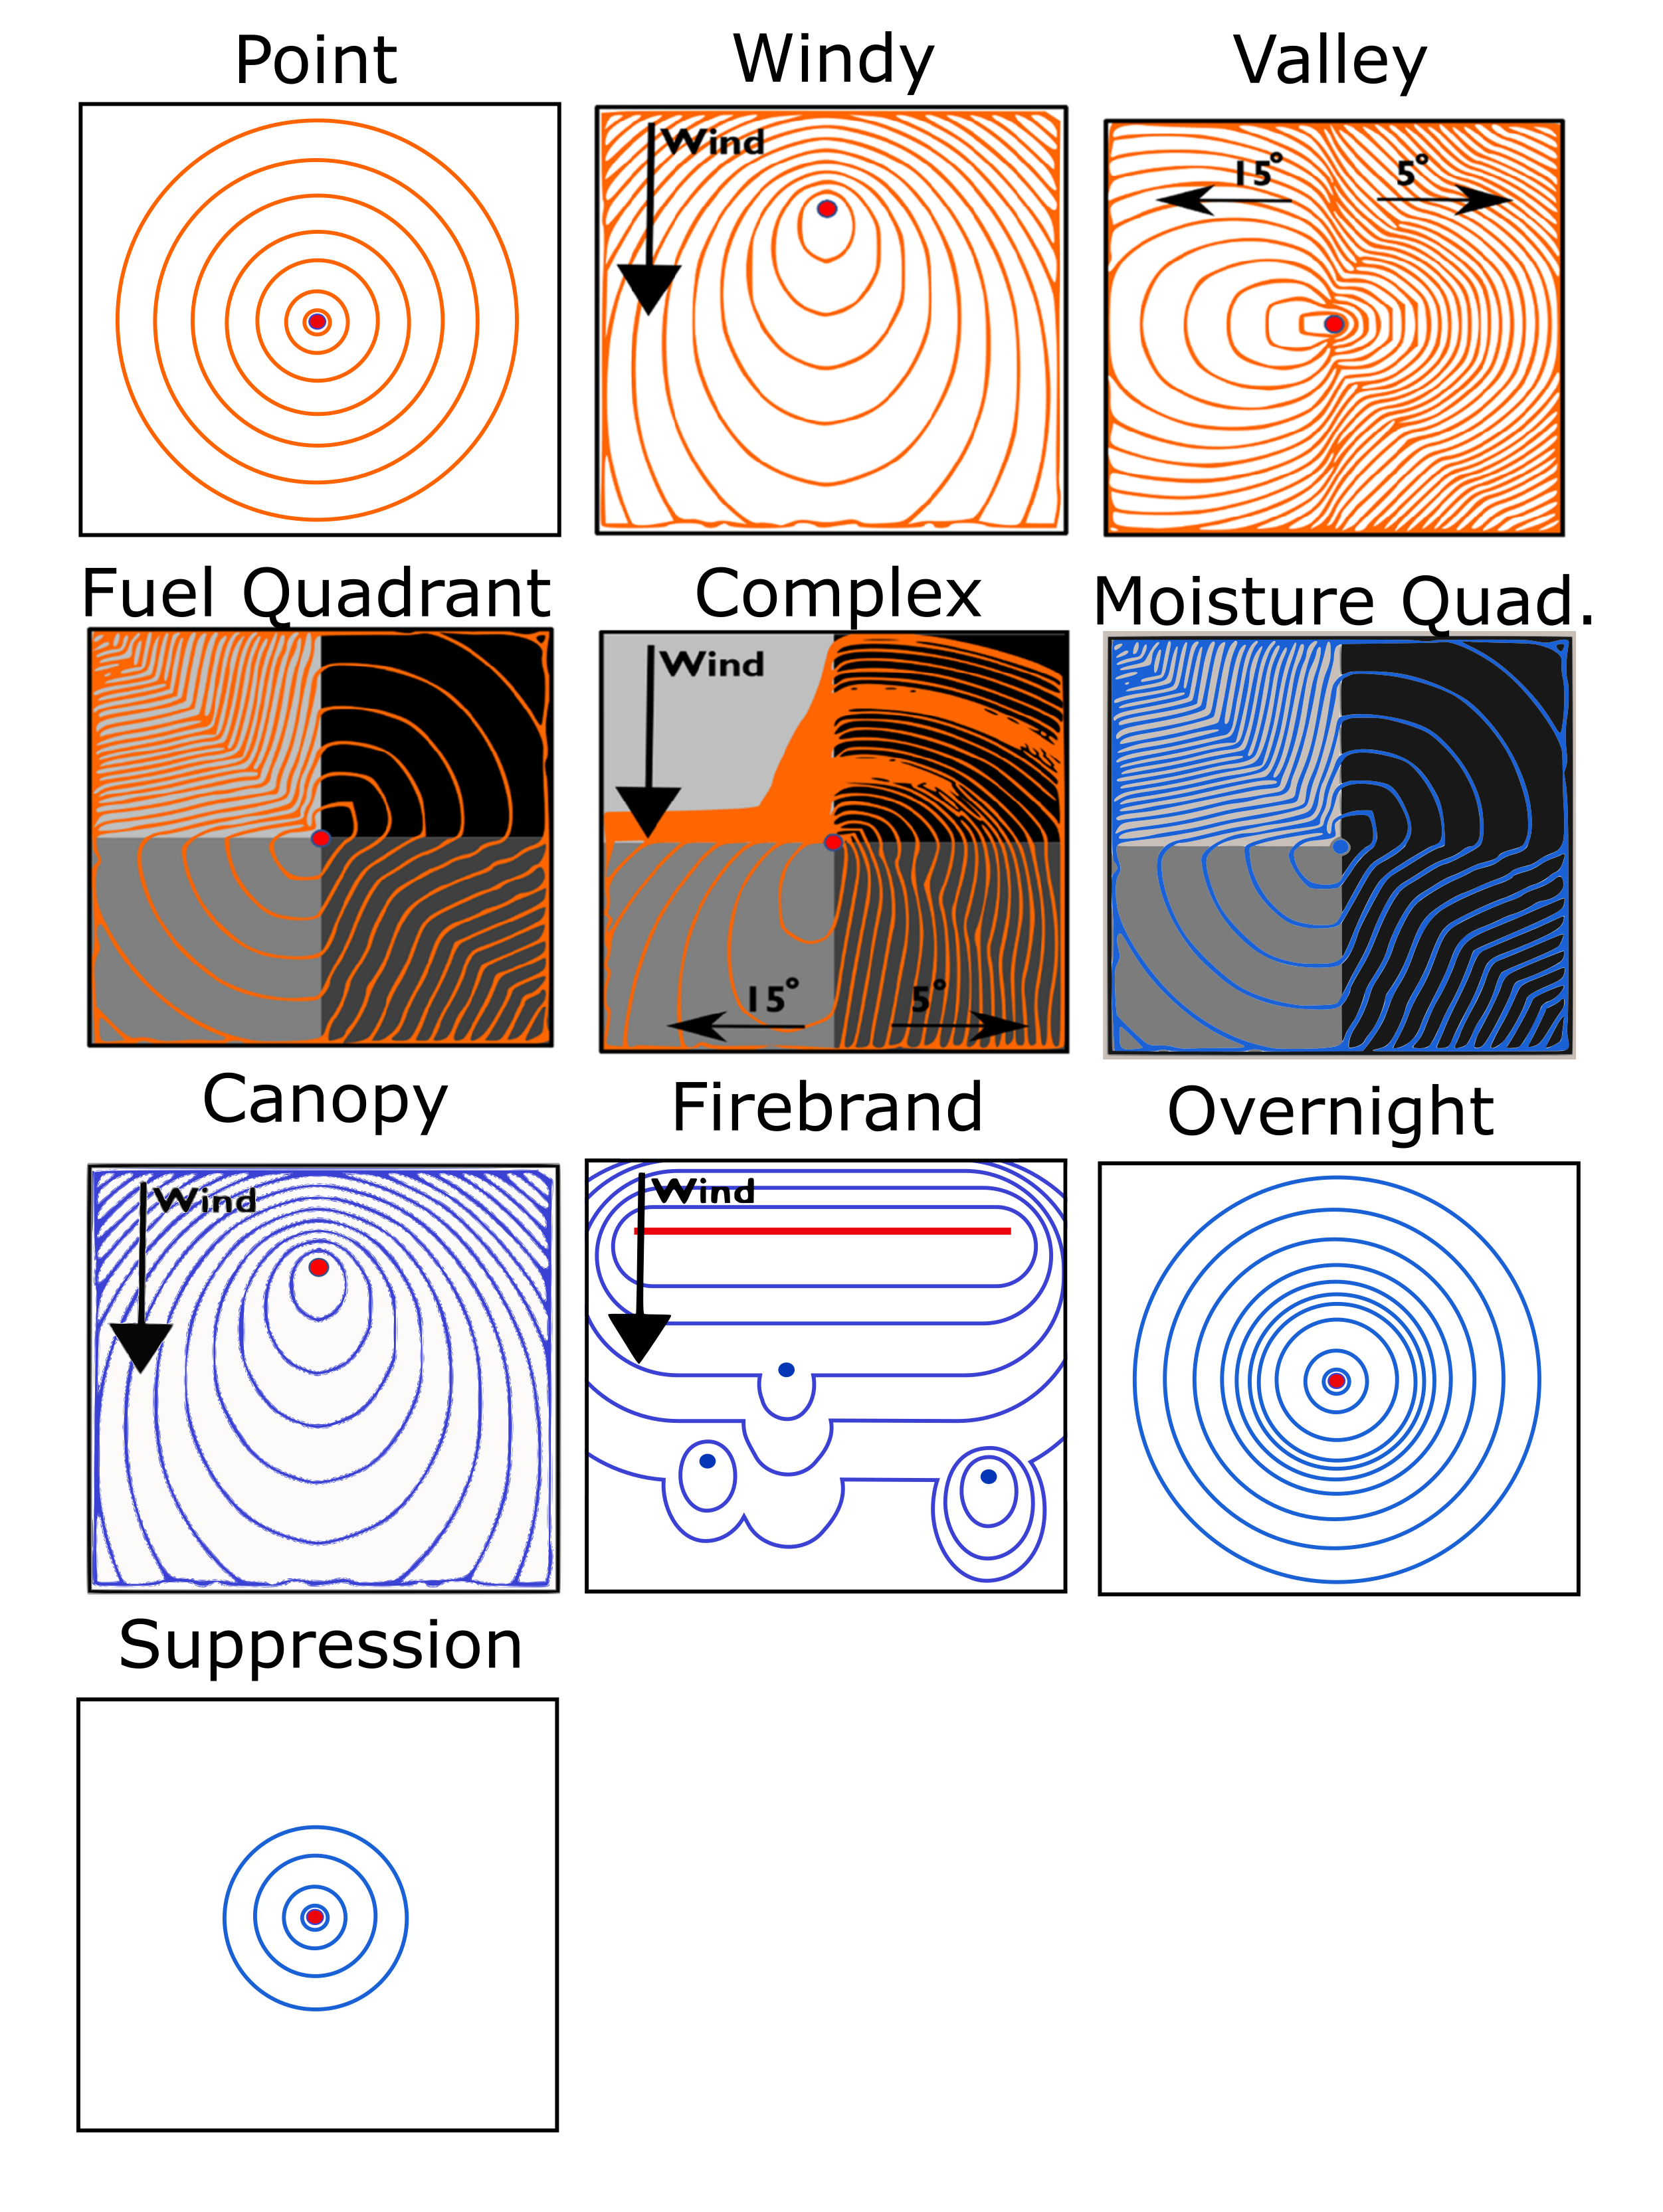
\includegraphics[width=0.8\linewidth]{figs/verification_cases.png}
 \caption{The nine verification cases of this study. The orange fire fronts represent the original five cases, and the blue fire fronts represent the new cases. Adapted from WUI-NITY 2.}
 \label{fig:verification_cases}
\end{figure}

The details of each case are described in Tab. \ref{tab:verification_params}. All the raster inputs are 126 x 126 cells with 30m cell size. Wind magnitude and direction is spatially constant. Simulation DT is 1 minute. Wind is specified at 10m height. 10-hour and 100-hour fuel moistures are 7\% and 8\% for all fuels and cases, live herbaceous fuel moisture is set to 90\% and live woody fuel moisture is set to 60\%. Where analytical solutions for the rate of spread can be acquired, they are calculated through the Rothermel model and the BEHAVE program. All isochrones shown in the later sections are hourly.

\begin{table}[t]
\centering
\caption{Simulation parameters of each verification case. Changes in fuel types between cases occur to generate faster or slower wildfires, for better visualisation or comparison.}
\label{tab:verification_params}

\begin{adjustbox}{max width=\textwidth}
\begin{tabular}{lccccccccccc}
\toprule
\textbf{Case} & 
\rotatebox{90}{\textbf{Topography}} & 
\rotatebox{90}{\textbf{Fuel (FBFM13)}} & 
\rotatebox{90}{\textbf{CC (\%)}} & 
\rotatebox{90}{\textbf{CBH (m×10)}} & 
\rotatebox{90}{\textbf{CBD (kg/m\textsuperscript{3}×100)}} & 
\rotatebox{90}{\textbf{CH (m×10)}} & 
\rotatebox{90}{\textbf{Wind (mph)}} & 
\rotatebox{90}{\textbf{1h FMC}} & 
\rotatebox{90}{\textbf{Firebrands}} & 
\rotatebox{90}{\textbf{Diurnal}} & 
\rotatebox{90}{\textbf{Suppression}} \\
\midrule
Point  & Flat & 3  & 0 & 0  & 0 & 0 & 0.0  & 6  & off  & off  & off \\
Windy  & Flat & 5  & 0 & 0  & 0 & 0 & 5  & 6  & off  & off  & off \\
Valley & 5° east, 15° west & 3  & 0 & 0  & 0 & 0 & 0.0  & 6  & off  & off  & off \\
Fuel Quadrant  & Flat & 8, 7, 4, 2 & 0 & 0  & 0 & 0 & 0.0  & 6  & off  & off  & off \\
Complex  & 5° east, 15° west & 8, 7, 4, 2 & 0 & 0  & 0 & 0 & 5  & 6  & off  & off  & off \\
Moisture Quad. & Flat & 3  & 0 & 0  & 0 & 0 & 0.0  & 6, 12, 18, 25 & off  & off  & off \\
Canopy & Flat & 5  & 80   & 16 & 16   & 55  & 6.0  & 6  & off  & off  & off \\
Firebrand   & Flat & 3  & 0 & 0  & 0 & 0 & 5  & 6  & on & off  & off \\
Overnight   & Flat & 3  & 0 & 0  & 0 & 0 & 0.0  & 6  & off  & 72 h runtime  & off \\
Suppression & Flat & 3  & 0 & 0  & 0 & 0 & 0.0  & 6  & off  & off  & on  \\
\bottomrule
\end{tabular}
\end{adjustbox}

\end{table}

\subsection{Point}

The first verification case tests ELMFIRE's ability to model simple fire spread. Under zero terrain changes and zero wind, flame spread is expected to be equal in all directions, forming circular fire fronts. The ELMFIRE output should be perfectly circular fire fronts, equidistant from each other, at a steady rate of spread. The Rothermel model, solved analytically through the BEHAVE program, predicts a maximum rate of spread of 1.51 m/min. Inputs to BEHAVE’s surface module are as follows:

\begin{itemize}
    \item Fuel Model: FB3 (3) Tall Grass (static)
    \item 1-h fuel moisture: 6\%
    \item 10-m wind speed: 0 mph
    \item Slope steepness: 0\%
\end{itemize}

The output of verification case ``Point'' is shown in Fig. \ref{fig:elm_point}. The estimated rate of spread of the fire is 4.96 ft/min, which is equal to 1.51 m/min, exactly matching the BEHAVE output. The output is perfectly circular, as expected from theory. 

\begin{figure}[h!]
    \centering
    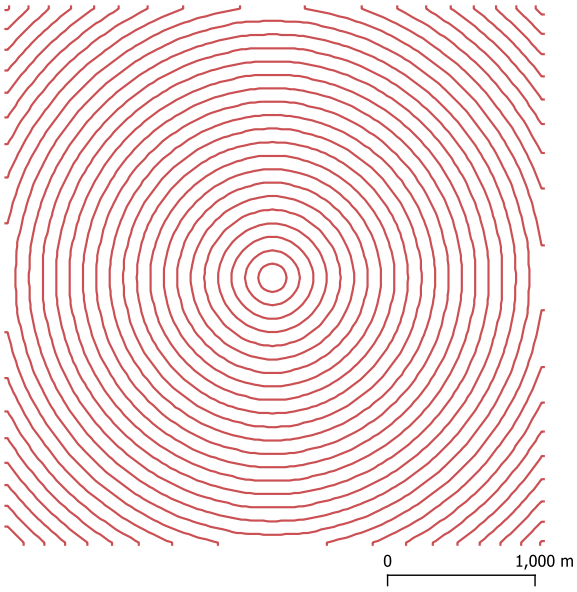
\includegraphics[width=0.6\linewidth]{figs/point.png}
    \caption{ELMFIRE simulation of verification case ``Point''}
    \label{fig:elm_point}
\end{figure}

\subsection{Windy}

While the previous case was a very simple test of fire spread, the ``Windy'' case tests the ability of ELMFIRE to adjust its maximum rate of spread accounting for wind, and its ability to spread wildfire in the landscape with heterogeneous wildfire spread. 

Now that wind is also involved, another parameter that needs to be solved and used as an input to BEHAVE is the wind adjustment factor. The wind adjustment factor is used to convert the free wind speed (20 ft) to midflame windspeed. It can be analytically calculated using the empirical relations of Andrews (2012) for an uncovered fuel (no or sparse canopy):

\begin{equation}
WAF_u = 
\frac{1.83}{
\ln\left(
\frac{20 + 0.36H}{0.13H}
\right)}
\end{equation}

Where H is the fuel depth height in feet. If canopy is present, the sheltered WAF is used. All WAF values are constrained between 0.1 and 1. 

\begin{equation}
WAF_s = 
\frac{0.555}{\sqrt{\frac{H(CH-CBH)}{CH}}
\ln\left(
\frac{20 + 0.36H}{0.13H}
\right)}
\end{equation}

The above equations can be rigorously solved, and in the case of uniform topography and constant wind can be solved to give the fire isochrone at a specific point in time. This analytical isochrone can be directly compared with the computational solution. The analytical solution can be derived with the help of BEHAVE, using the following parameters:

\begin{itemize}
    \item Fuel Model: FB5 (5) Brush (static)
    \item 1-h fuel moisture: 6\%
    \item 10-h fuel moisture: 7\%
    \item 10-m wind speed: 6 mph
    \item Slope steepness: 0\%
    \item Wind adjustment factor: 0.418
\end{itemize}

The above yields:

\begin{itemize}
    \item Head rate of spread: 3.06 m/min
    \item Backing rate of spread: 0.88 m/min
    \item Midflame windspeed: 3.5 km/h
    \item $L/W$: 1.20
\end{itemize}

ELMFIRE then predicts:

\begin{itemize}
    \item Head rate of spread: 3.07 m/min
    \item Backing rate of spread: 0.88 m/min
    \item $L/W$: 1.21
\end{itemize}

The above results can be confirmed visually in Fig. \ref{fig:elm_windy}. The exact solution and the simulated solution are a near exact match. This proves that the elliptical fire spread in ELMFIRE works as intended, and the model overall can accurately model simple wind-driven fires. 

\begin{figure}[h]
    \centering
    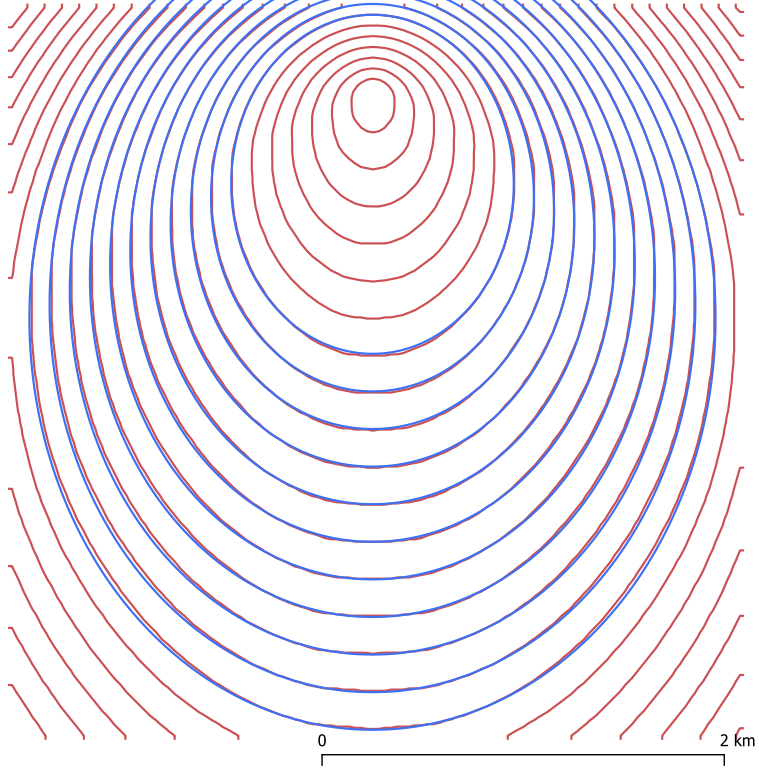
\includegraphics[width=0.6\linewidth]{figs/windy.png}
    \caption{ELMFIRE Simulation (red) of verification case ``Windy''. Analytical solutions (blue) superimposed.}
    \label{fig:elm_windy}
\end{figure}

\subsection{Valley}

 Since slope and wind are treated similarly in the 2D spread calculations, both being added to the vector quantity $\phi$ before being used in the equations presented in the previous chapter, a similar analysis to the ``Windy'' case will not be conducted as it would not provide any new verification to the model. The Rate of Spread values will be compared to behave as before, and instead the Huygens principle will be tested, by comparing successive isochrones of the simulated fire to the earlier isochrone's individual point-source expansions. Using BEHAVE with:

 \begin{itemize}
    \item Fuel Model: FB3 (3) Tall Grass (static)
    \item 1-h fuel moisture: 6\%
    \item 10-m wind speed: 0 mph
    \item Slope steepness: 5\% / 15\%
\end{itemize}

The above yields:

\begin{itemize}
    \item Head rate of spread (5\%): 1.92 m/min
    \item $L/W$ (5\%): 1.01
    \item Head rate of spread (15\%): 5.37 m/min
    \item $L/W$ (15\%): 1.07
\end{itemize}

ELMFIRE then predicts:

\begin{itemize}
    \item Head rate of spread (5\%): 1.92 m/min
    \item Head rate of spread (15\%): 5.37 m/min
\end{itemize}

Calculating the $L/W$ of each slope from these complex isochrones is not straightforward, so instead the inverse is done. BEHAVE is used to get the $L/W$ of the two parts of the landscape, and 1-hour contours of each part are drawn. Those 1-hour contours are placed on one isochrone, to test if the resulting controur matches the next isochrone, as per Huygens' principle. 

\begin{itemize}
    \item Head $L/W$ (5\%): 1.01 
    \item Head $L/W$ (15\%): 1.07
\end{itemize}

Creating 1-hour point spreads and overlapping them to one isochrone should overlap with the next outline in ELMFIRE. Indeed, plotting the point spreads with the same function as ``Windy'' yields satisfactory results.

\begin{figure}[h!]
    \centering

    \begin{subfigure}[b]{0.48\linewidth}
        \centering
        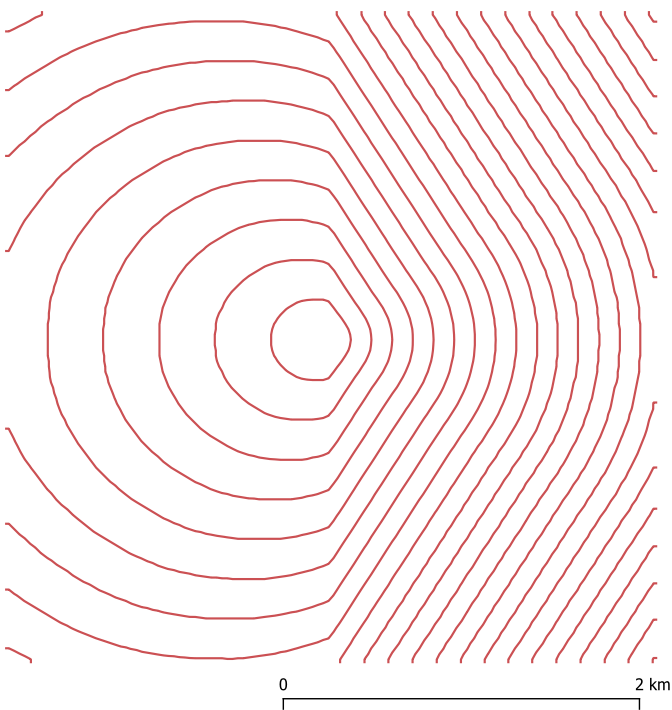
\includegraphics[width=\linewidth]{figs/valley.png}
        \caption{}
    \end{subfigure}
    \hfill
    \begin{subfigure}[b]{0.48\linewidth}
        \centering
        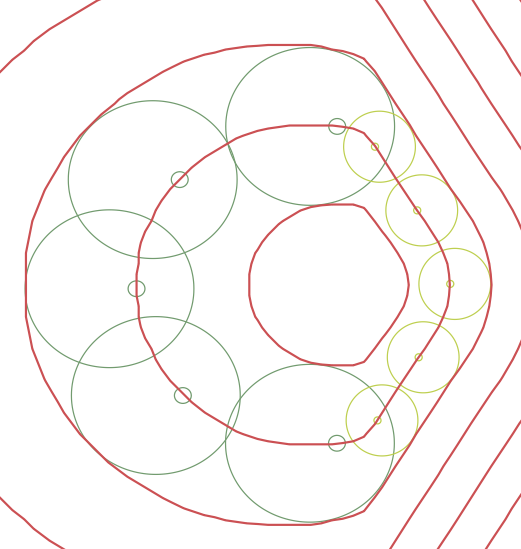
\includegraphics[width=\linewidth]{figs/valley_huygens.png}
        \caption{}
    \end{subfigure}

    \caption{Left: The ``Valley'' verification case in ELMFIRE. Right: the 5° and 15° incline point ignition ellipses overlapped between two isochrones, with great match.}
    \label{fig:elm_valley}
\end{figure}

\subsection{Quadrant}

This scenario tests multiple fuel models at the same time, which can be used to ensure that the resulting complex contour are physically realistic and that the resulting rate of spread for each fuel matches the BEHAVE output. 

Using BEHAVE:

\begin{itemize}
    \item Fuel Model:
    \begin{enumerate}
        \item FB2 (2) Timber (grass and understory)
        \item FB4 (4) Chaparral (6 feet)
        \item FB7 (7) Southern Rough
        \item FB8 (8) Closed Timber Litter
    \end{enumerate}
    \item 1-h fuel moisture: 6\%
    \item 10-h fuel moisture: 7\%
    \item 100-h fuel moisture: 8\%
    \item Live herbaceous fuel moisture: 60\%
    \item Live woody fuel moisture: 90\%
    \item 10-m wind speed: 0 mph
    \item Slope steepness: 0\%
\end{itemize}

Results in:

\begin{enumerate}
    \item FB2 Head Rate of Spread: 0.871 m/min
    \item FB4 Head Rate of Spread: 1.492 m/min
    \item FB7 Head Rate of Spread: 0.472 m/min
    \item FB8 Head Rate of Spread: 0.080 m/min
\end{enumerate}

ELMFIRE then predicts:

\begin{enumerate}
    \item FB2 Head Rate of Spread: 0.872 m/min
    \item FB4 Head Rate of Spread: 1.974 m/min
    \item FB7 Head Rate of Spread: 0.551 m/min
    \item FB8 Head Rate of Spread: 0.080 m/min
\end{enumerate}

.......................................

\subsection{Complex}

The complex case is beyond analytical solution or comparison to an ideal solution and is the primary reason why one needs wildfire spread models. This case is added for qualitative review, to showcase the compilation of previous cases and investigate whether the results do linearly add to one another. As such, it is expected to see fast southward spread, with higher spread eastward (toward the higher slope) and towards the faster-spread fuel model. Indeed, that is exactly what ELMFIRE predicts. 

\begin{figure}[h!]
    \centering
    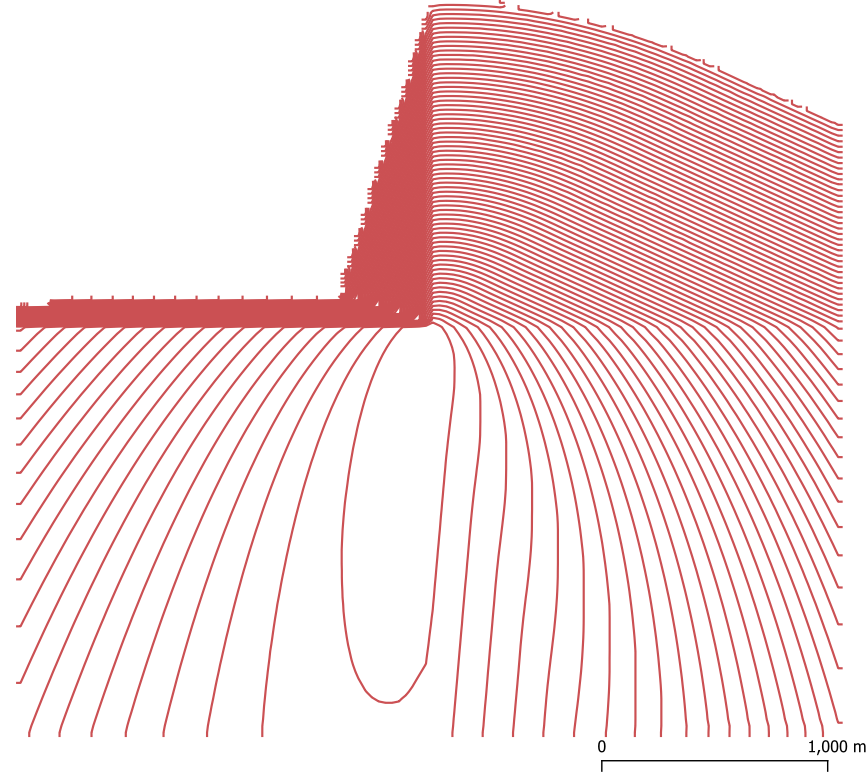
\includegraphics[width=0.6\linewidth]{figs/complex.png}
    \caption{The ``Complex'' verification case results from ELMFIRE.}
    \label{fig:elm_complex}
\end{figure}

\subsection{Moisture Quad}

In this verification scenario, a landscape of uniform fuel is used, where each quadrant has different fuel moisture content. This test ensures that the fuel moisture content values are correctly interpreted by ELMFIRE. One of the moisture values (25\%) is equal to the moisture of extinction of fuel model 3. As such, it is expected to have zero fire spread within that area of the raster. Once again, the results will be compared to the outputs of BEHAVE. Those are calculated by using:

\begin{itemize}
    \item Fuel Model: FB3 (3) Tall grass (static)
    \item 1-h fuel moisture: 6\%, 12\%, 18\%, 25\%
    \item 10-m wind speed: 0 mph
    \item Slope steepness: 0\%
\end{itemize}

The BEHAVE results then are:

\begin{enumerate}
    \item 6\%: 1.511 m/min
    \item 12\%: 1.089 m/min
    \item 18\%: 0.801 m/min
    \item 25\%: 0 m/min
\end{enumerate}

ELMFIRE consequently predicts:

\begin{enumerate}
    \item 6\%: 1.511 m/min
    \item 12\%: 1.089 m/min
    \item 18\%: 0.801 m/min
    \item 25\%: 0 m/min
\end{enumerate}

The ELMFIRE results are identical to those predicted in BEHAVE, verifying that ELMFIRE correctly parses fuel moisture values. Note that in this case only the 1-hour fuel moisture values were spatially varied; rate of spread is influenced by a mixture of the different available fuel moisture values, depending on the fuel type. The 1-hour fuel type is majorly responsible for setting the rate of spread of all the fuels, so ensuring that it works can be considered enough for this verification.

\begin{figure}
    \centering
    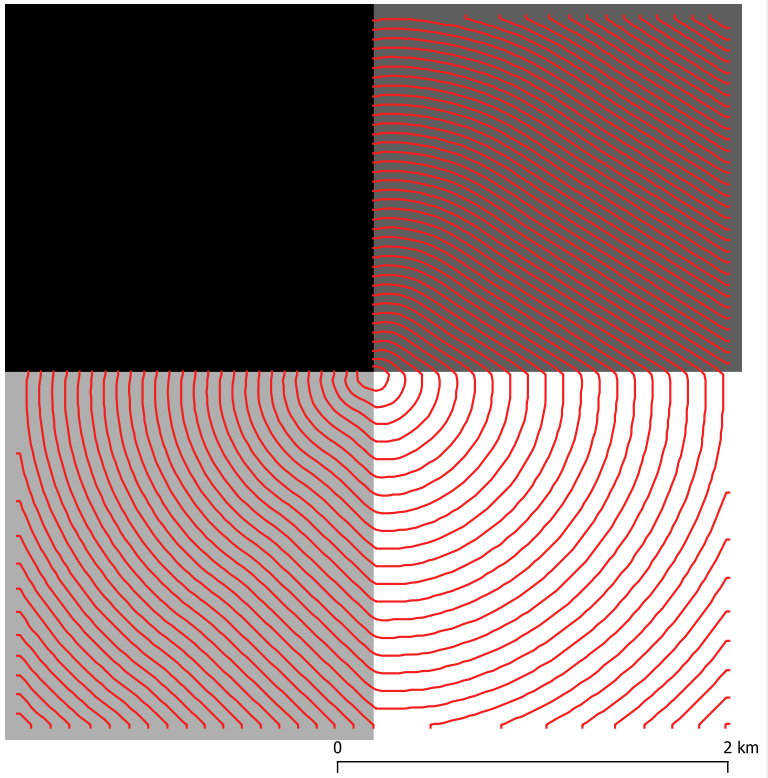
\includegraphics[width=0.6\linewidth]{figs/moisturequad.png}
    \caption{The ``Moisture Quadrant'' verification case results in ELMFIRE. Fuel moisture is plotted on the background with values ranging from 6 (white) to 25 (black).}
    \label{fig:elm_moistquad}
\end{figure}

\subsection{Canopy}

This verification scenario introduces nonzero canopy values to the simulation, to investigate the effect it introduces to the rate of spread of the fire. Theory dictates that a surface fire may ignite the canopy and start a passive, active or independent crown fire depending on the canopy conditions and the surface intensity of the fire. Independent crown fire behavior, where the canopy fire can progress uncoupled from the surface fire, is not modelled in ELMFIRE. BEHAVE can no longer be used directly in this verification step, since it uses a different crown fire calculation model. It can be used to provide the initial rate of spread and fireline intensity values. In BEHAVE:

\begin{itemize}
    \item Fuel Model: FB5 (3) Tall Grass (static)
    \item 1-h fuel moisture: 6\%
    \item 10-m wind speed: 6 mph
    \item Slope steepness: 0\%
    \item Wind adjustment factor: 0.1
\end{itemize}

Results in:

\begin{itemize}
    \item No-wind, no-slope rate of spread ${R_{R,0}}$: 1.511 m/min
    \item Head rate of spread: 3.475 m/min
    \item Fireline Intensity $I_b$: 488.6 kW/m
\end{itemize}

Plugging in these values to the above equations yields:

\begin{itemize}
    \item Critical crown rate of spread $R_0$: 18.75 m/min
    \item Predicted crown rate of spread $R_C$: 21.5 m/min
    \item Critical Fireline Intensity $I_0$: 298.4 kW/m
\end{itemize}

Hence, in this situation, the surface fire would have sufficient energy to ignite the canopy, and the fire would turn to an active crown fire. Indeed, ELMFIRE predicts parts of the head fire undergoing active crown fire:

\begin{itemize}
    \item Head rate of spread (Active): 21.3 m/min
\end{itemize}

In very good agreement with the theoretical output.

This verification case was repeated for wind magnitude of 2 mph. The analytical solution then is:

\begin{itemize}
    \item No-wind, no-slope rate of spread ${R_{R,0}}$: 1.511 m/min
    \item Head rate of spread: 1.976 m/min
    \item Fireline Intensity $I_b$: 277.92 kW/m
    \item Critical crown rate of spread $R_0$: 18.75 m/min
    \item Predicted crown rate of spread $R_C$: 8.0 m/min
    \item Critical Fireline Intensity $I_0$: 298.4 kW/m
\end{itemize}

The surface fire would have insufficient energy to start a crown fire. ELMFIRE predicts no crown fire, and:

\begin{itemize}
    \item Head rate of spread: 1.96 m/min
    \item Fireline Intensity $I_b$: 280.3 kW/m
\end{itemize}

In good agreement with BEHAVE. A final simulation at 3 mph was conducted, which according to the analytical calculations, should result in a passive crown fire:

\begin{itemize}
    \item No-wind, no-slope rate of spread ${R_{R,0}}$: 1.511 m/min
    \item Head rate of spread: 2.303 m/min
    \item Fireline Intensity $I_b$: 323.81 kW/m
    \item Critical crown rate of spread $R_0$: 18.75 m/min
    \item Predicted crown rate of spread $R_C$: 11.5 m/min
    \item Critical Fireline Intensity $I_0$: 298.4 kW/m
    \item Passive crown fire rate of spread: 6.2 m/min
\end{itemize}

ELMFIRE agrees with the above, predicting a passive crown fire towards the head fire, and no crown fire in the flank and backfires. This makes sense since the fireline intensity is less and may not be sufficient to ignite the canopy/.

\begin{itemize}
    \item Head rate of spread: 6.1 m/min
\end{itemize}

Which is equal to the predicted passive crown fire rate of spread. 

\begin{figure}
    \centering
    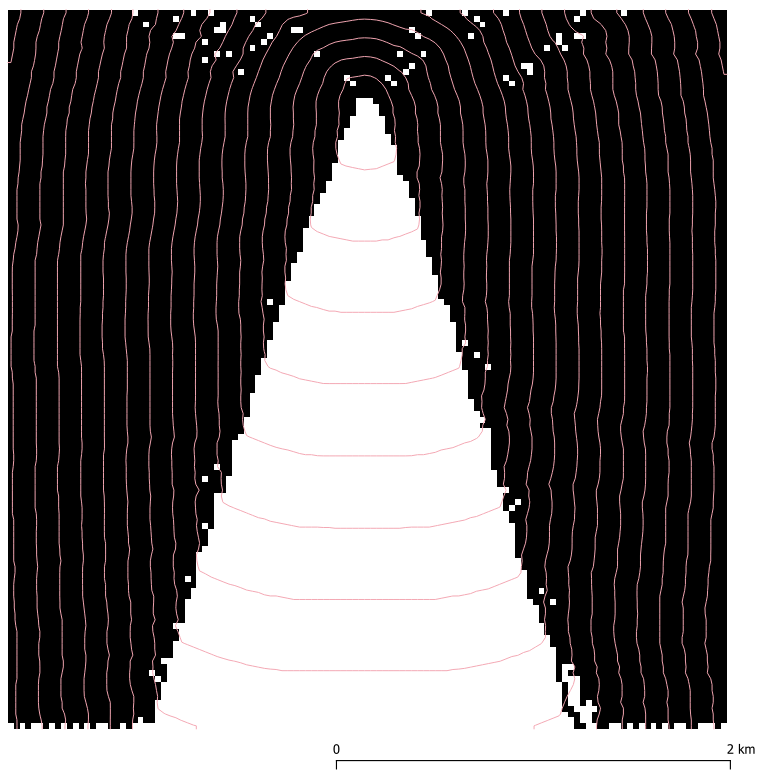
\includegraphics[width=0.45\linewidth]{figs/canopy_passive.png}
    \caption{The ELMFIRE results of the ``Canopy'' verification with 3 mph wind. White parts of the landscape are undergoing passive crown fire, and black parts do not have crown fire.}
    \label{fig:placeholder}
\end{figure}

As such, ELMFIRE can be considered verified for crown fire spread classification and calculation.

\subsection{Firebrand}

Firebrand generation, referred to as Spotting within ELMFIRE, controls the generation of small particles capable of creating new ignition sources downwind of the fire, accelerating the effective fire front. ELMFIRE has a multitude of different modes for firebrand spread, depending on the stage of calculation. There are three different models for generation, transport, and ignition. There are also differences in whether the firebrands are solves as discrete particles (lagrangian) or as fluxes on a grid (eulerian).

Firebrand generation in ELMFIRE can either be controlled explicitly through maximum and minimum limits, implicitly through a ember generation factor per square meter per minute, or physically through the fireline intensity and a parameterised generation constant. All of these methods are simple and straightforward enough that verification is not a required step. 

Firebrand transport can be set by the user as uniform (between a max and min value), lognormal (with a specific mean and standard deviation), and Sardoy (precomputed lognormal distribution). The Sardoy model follows the parameterisation of \cite{sardoy_numerical_2008} and will not be covered in depth here. The lognormal distribution application, which is used when the Sardoy model is specified, should be validated as it requires a series of steps to be computed. A simulation that includes firebrands will generate a spotting\_stats\_0000001.csv file with a log of specific firebrand trajectory and statistics. Those include the distance travelled by each firebrand, their origin, destination and loft time, and the fireline intensity of the generation cell. A sample of the table is given in \ref{tab:verif-embers-distance}. The last column is calculated from the input data and the mathematical details in \ref{ember_transport}. The calculated values match exactly with the simulated values, meaning the transport part of ELMFIRE can be considered validated. 

\begin{table}[]
\caption{A part of the firebrand verification case with lognormal distribution distances. The last column is calculated based on the Mathematical section details. }
\label{tab:verif-embers-distance}
\begin{tabular}{llllllllll}
IX\_FROM & IY\_FROM & IX\_TO & IY\_TO & TLAUNCH & TIGN   & DIST  & FLIN   & CALCULATED DIST & DIST DIFFERENCE \\
63      & 109     & 63    & 105   & 121.35  & 224.2  & 96.51 & 1656.6 & 96.5            & 0.0             \\
63      & 108     & 63    & 104   & 409.71  & 512.57 & 96.51 & 1656.6 & 96.5            & 0.0             \\
62      & 109     & 62    & 106   & 409.71  & 486.85 & 85    & 1285.0 & 85.0            & 0.0             \\
64      & 109     & 64    & 106   & 409.71  & 486.85 & 85    & 1285.0 & 85.0            & 0.0             \\
63      & 104     & 63    & 100   & 467.38  & 570.24 & 96.51 & 1656.6 & 96.5            & 0.0             \\
62      & 108     & 62    & 104   & 582.73  & 685.59 & 91.7  & 1495.6 & 91.7            & 0.0             \\
64      & 108     & 64    & 104   & 582.73  & 685.59 & 92.2  & 1511.9 & 92.2            & 0.0             \\
63      & 103     & 63    & 99    & 698.08  & 800.93 & 96.51 & 1656.6 & 96.5            & 0.0             \\
62      & 104     & 62    & 101   & 698.08  & 775.22 & 85.25 & 1292.6 & 85.3            & 0.0            
\end{tabular}
\end{table}

The transport and accumulation (and thus ignition) mechanisms of firebrands is different for the lagrangian and eulerian approaches. With the largangian model, the ignition probability is an explicit input variable that applies to each landed firebrand. It does not require verification due to the simplicity of its application. The eulerian model is more complicated and requires verification.

For the eulerian model verification case the most complicated model settings have been chosen by enabling USE\_PHYSICAL\_EMBER\_NUMBER to physically estimate generation, USE\_UMD\_SPOTTING\_MODEL to physically estimate transport, and USE\_SIMPLE\_IGNITION\_MODEL = .FALSE. (which requires USE\_EMBER\_IGNITION\_MODEL) to physically estimate ignition. This way, a minimal number of variables need to be set by the user, namely just CROWN\_FIRE\_SPOTTING\_PERCENT.

The final parameter that will be used for verification is the ember flux on a single cell. A cell in the centerline of the symmetrical domain is chosen (identical to the Canopy case), and thus the mathematical analogue for verification can be treated as 1D. In 1D, and assuming steady state, each cell has the same firebrand generation and transport profile. 

The input conditions of each cell are (taken as an approximate average of the main fire front:

\begin{itemize}
    \item 20ft wind speed ($U_{20}$): 1.341 m/s
    \item Fireline Intensity ($I_b$): 260 kW/m
    \item Timestep duration ($\Delta t$): 189.7 s
    \item Cellsize ($C$): 30 m
    
\end{itemize}

The total ember count emitted from the cell is calculated by:

\[
N=0.0333\Delta T \;I_b\;C
\]

With 0.0333 being an empirical constant of firebrands per kW. The above results at a total firebrand count of 49280. ELMFIRE calculates values approximately close to 49500, in close agreement with the mathematical expectation. 


Then, to choose the appropriate set of equations to find total travel distance, the Froude number is calculated by:

\[
Fr = \frac{U_{20}}{\sqrt{gL_c}}\;\;\;\;\;Lc=\frac{I_b}{\rho_\infty C_{pg} \tau_\infty \sqrt{g}}
\]

The values $g=9.81$, $\rho_\infty = 1.1$, $C_{pg} = 1$, and $\tau_\infty = 300$ are constants. 

The above result in $L_c = 1.36 m$ and $Fr = 0.37$

Thus the travel distance parameters downwind ($\mu_d, \;\sigma_d$) and spanwise ($\mu_s, \;\sigma_s$) of the source are calculated:

\[
\mu_d=1.47\frac{(0.001I_b)^{0.54}}{U_{20}^{0.55}}+1.14
\]
\[
\sigma_d=0.86\frac{U_{20}^{0.44}}{(0.001I_b)^{0.21}}+0.19
\]
\[\mu_s=0\]
\[\sigma_s=0.92L_C\]

To then computationally solve the ember distribution, we require an upper value, set as the top 1\% of the Sardoy density function. The top 1\% distance is found through:

\[
D_d=\exp{[\mu_d+s\sigma_d]}
\]

\[
s = \sqrt{2}erf^{-1}(2 \times(1-0.01)-1)=2.32
\]

Then, $D_d=182.5 \;m $. Similarly for the spanwise ember spread, $D_s=0.87\;m$. This means that the ember distribution will be calculated for $nint(182.5/30)-1=5$ cells ahead of the source, and 0 cells spanwise. 

Then, for each cell downwind of the embers, the ember flux contribution from the source cell $Q_e$is:

\[
Q_e=P_L\;N
\]

With $P_L$ being the probability of ember deposition at the target cell. It is calculated through the Sardoy CDF, written in full below, with $d$ being the distance of the target cell downwind from the source cell.

\[
CDF_S(d, d-C)=0.5 \left(1+erf\left[\frac{ln(d-\mu_d)}{\sqrt{2}\sigma_d}\right]\right) - 0.5\left(1+erf\left[\frac{ln(d-C-\mu_d)}{\sqrt{2}\sigma_d}\right]\right)
\]

Then,

\[
P_d=\frac{CDF_S(d, d-C)}{CDF_S(D_D,0)}
\]

In the example we are solving for, any given source cell would emit:

\begin{itemize}
    \item 1st cell downwind: 43175 
    \item 2nd cell downwind: 3766
    \item 3rd cell downwind: 1250
    \item 4th cell downwind: 578
    \item 5th cell downwind: 316
\end{itemize}

Then, to solve for a given target cell, the ember flux needs to be summed for all the upwind source cells. These values can be compared with ELMFIRE outputs. For a given cell:

\begin{itemize}
    \item Target 5 cells from closest emitter (1 source): 316 (ELMFIRE: 364)
    \item Target 4 cells from closest emitter (2 sources): 894 (ELMFIRE: 731)
    \item Target 3 cells from closest emitter (3 sources): 2145 (ELMFIRE: 1744)
    \item Target 2 cells from closest emitter (4 sources): 5911 (ELMFIRE: 5753)
    \item Target 1 cell from closest emitter (5 sources): 49086 (ELMFIRE: 41967)
\end{itemize}

The ELMFIRE outputs are for a sample cell and may vary depending on the actual fireline intensity at each cell. The discrepancy between predicted and actual values is noticeable with large ember values, but is still within acceptable values considering the limitations of the analytical calculation input data. From this, the eulerian transport model of ELMFIRE and its associated submodules can be considered verified.

For ignition, ELMFIRE includes three different methods. With the lagrangian transport model, the user can set a direct change of ignition per firebrand, which does not require verification. With the eulerian transport model, the user can choose between a simple and a physical ignition model. The simple ignition model only depends on the user-set ignition probability (for any ember flux greater than zero) and the ratio of firebrand ignition delay and elmfire timestep. Using the physical model, the probability of ignition is then controlled by the firebrand coverage density, through experimental correlations. If the resulting condition exceeds a specific ignition criterion, ignition probability is set to 0.9, and zero otherwise. There is no verification method for this part of ELMFIRE at this time. 

\subsection{Overnight}

The verification cases are set at the equator and span multiple simulated hours; the ``Point'' case in particular has been set to run for 2 simulated days. In reality, wildfire slow down or even extinguish completely at night, where fuel humidity rises and winds die down. For this phenomenon to be accurately modelled, the fine fuel moisture should be interpolated using a diurnal weather profile. This way the fire spread can organically be influenced by the higher relative humidity that occurs at night. 

ELMFIRE does not adjust the 1-h fine fuel moisture once it is read as an input. To retain the effect of night-time slowing down, a constant factor of 0.1 is used to scale down the predicted rate of spread. This scaling occurs during the hours between sunset and sunrise. These hours are calculated in ELMFIRE through the NOAA Solar Position Calculations (too extensive to repeat here). For our test case, located at the equator, the sunrise and sunset times should be at 06:00 and 18:00 respectfully, regardless of the time of year. The simulation is made to start at 10:00. With a burn period length of 10 hours and a center fraction of 0.667, the expected hours that the overnight adjustment factor applies are between 19:00 and 11:00. 

The results of turning this option on is shown below. 

\begin{figure}[h!]
    \centering
    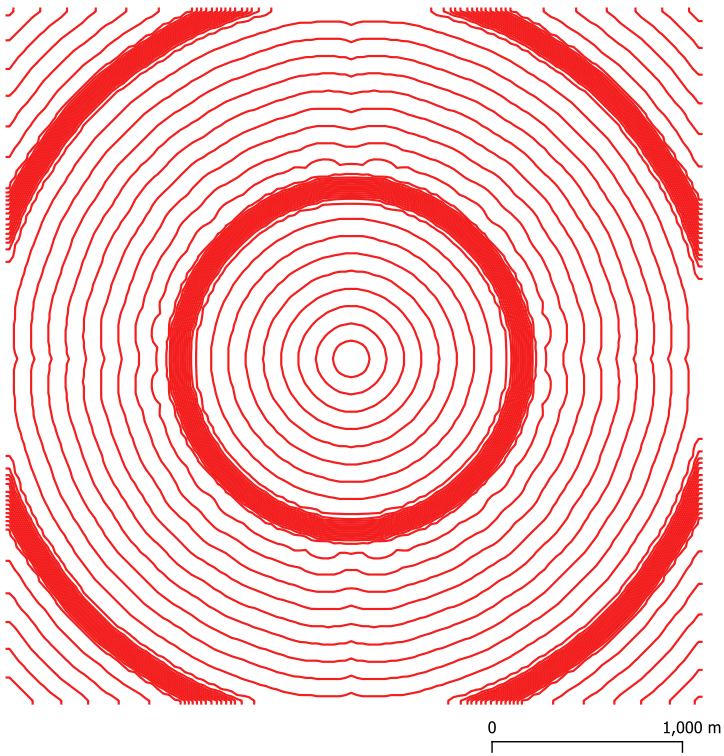
\includegraphics[width=0.6\linewidth]{figs/overnight.png}
    \caption{The results of the ``Overnight'' verification case.}
    \label{fig:elm_overnight}
\end{figure}

To make sure that ELMFIRE has calculated the times correctly, each isochrone is counted:

\begin{figure}
    \centering
    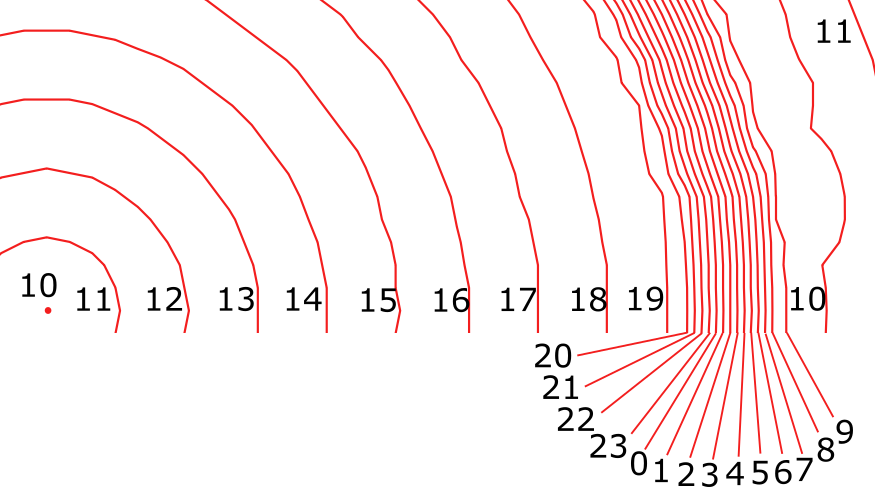
\includegraphics[width=0.5\linewidth]{figs/diurnal.png}
    \caption{An isochrone count of the Overnight verification case, with hours of arrival labelled on.}
    \label{fig:placeholder}
\end{figure}

The isochrone times are a close match with the expected slowdown and speed up times, hence ELMFIRE does correctly calculate the sunrise and sunset hours and apply the diurnal correction factor.

\subsection{Suppression}

Suppression includes the initial attack verification and the extended attack verification.

The initial attack submodel prescribes a probability of successful fire containment at the first attack opportunity. The final result is then compared to a random number and the simulation is either allows to continue or stop. For this verification case, the ``Point'' case will be used. The initial attack time is set to 4800 seconds. The rate of spread of the fire was calculated to be 1.51 m/min, meaning in 3600 seconds, the radius of the fire will be 120.8 m , and the total fire area will be 45800 $m^2$, or 11.3 acres. The acreage that ELMFIRE will use will be different because of the difference between the exact solution and the quantised solution (due to the large cell size). To find the value ELMFIRE uses, we find all cells in the solved ``Point'' case with arrival time less than 4800 s. The total cell count is 69, with a total area of 62100 $m^2$, or 15.3 acres, or 6.2 hectares. The fireline intensity of the same case is 212.5 kW/m. 

With the above values, the probability of containment will be 54\%. To test this, the Initial Attack verification case has been set up to run 20000 simulations with the same parameters and a new random seed every time. The resulting fire size stats should show whether the fire stops early or burns through the landscape. Totaling the results, about 52\% of the simulated fires are contained at the time of the initial attack, adequately close to the predicted value.

For the extended attack verification case, the same case as ``Point'' will be ran again, this time with ENABLE\_EXTENDED\_ATTACK = .TRUE., and all the values left as standard. Since this is a simple circular case, the containment equations can be solved analytically. 

The area change every hour for the verification case is:

\[
\frac{\delta A}{\delta T}=\frac{\pi(R_T^2-R_{T-\Delta T}^2)}{\Delta T}=\frac{\pi U^2[T^2 - (T-\Delta T)^2]}{\Delta T}=\pi U^2 (T-\Delta T)
\]

Where, different from the nomenclature of the rest of the guide, $R$ is the radius of the circular fire scar, $U$ is the rate of spread of the fire, $T$ is the current time and $\Delta T$ is the suppression time step. Since a spatial SDI is not give, a default value of 1 is used. Then, the change in containment per time step is:

\[
\delta C_{T,t}=0.01\psi C_mJ\exp{(-|B_{SDI}\overline{SDI}_t|)} = 0.01*1*100*\left(1-\frac{\delta A/\delta t}{10000}\right)*\exp{(-|1*1|)}=0.34\left(1-\frac{\pi U^2 (T-\Delta T)}{10000}\right)
\]

Plugging in known values yields:

\[
\delta C_{T,t}=0.34\left(1-\frac{\pi 1.51^2 (T-3600)}{10000}\right)
\]

This equation can be solved analytically per time step:

\begin{itemize}
    \item $T = 3600$, $\delta C_{T,3600}=0.3678$, $C_T=0.3678$
    \item $T = 7200$, $\delta C_{T,7200}=0.3671$, $C_T=0.7350$
    \item $T = 10800$, $\delta C_{T,10800}=0.3667$, $C_T=1.101$
\end{itemize}

As such, the simulation is expected to end at a time of 10800 seconds. Indeed, the simulation stops at a time ~10000 seconds, with a final containment of 1. The final time is taken from the arrival time raster, as the fire stats output may return the inaccurate simulation end time. 

\section{FBP Test Cases}

The 2009 update to the FBP system \cite{wotton_updates_2009} contained a set of 20 verification cases, to specifically test implementations of FBP in new models or fire spread codes. Each test varies the fuel model, wind and slope vectors, fine fuel moisture contents, and other parameters to test the correct implementation of each part of the system. The 2009* update also provides final and intermediate scalar values of the fire parameters (spread rate, fireline intensity, and fuel consumption of the surface and canopy respectively). These provided tests, and the accompanying tables of results, were instrumental in the implementation and testing of the FBP module of ELMFIRE, and the developers want to thank the authors for their foresight and for providing these cases.

As only the head fire model has been implemented in ELMFIRE, the results ignore the flank and backfire part of the FBP model, as it was not implemented. The 20 cases have been implemented in ELMFIRE and can be ran automatically, with a final verdict on the similarity of the results. At present, the maximum head rate of spread and fireline intensity are tested. a 10\% error window has been introduced to allow for the effect of rounding errors (e.g. between the listed slope rise given in percent and the slope input ELMFIRE accepts in nearest integer degree). 

The results are given in the table below. All tests can be found in the verification folder of ELMFIRE. To run these tests, navigate to \verb|\elmfire\verification\FBP_tests\| and run \verb|./runme.sh|. The script will clear existing results, produce the ELMFIRE input files and case folders, run ELMFIRE for each case, and compare the results with the ones in the 2009 Update. A 10\% margin of error is included to account for differences in slope definition and other accuracy differences between ELMFIRE integer inputs and the float inputs. As standard, the level set mode results will be displayed, but the fire potential mode results can also be compared by running  \verb|python compare.py --mode 2| (some python packages might need to be installed through pip / conda).

\begin{table}[h!]
\centering
\begin{tabular}{r r r r r r r c c}
\hline
Run & $ROS_{target}$ & $ROS_{sim}$ & $ROS_{error}\% $ & $FI_{target}$ & $FI_{sim}$ & $FI_{error}$\% & $ROS_{match}$ & $FI_{match}
$ \\
\hline
01 & 5.6  & 5.3  & -4.6 & 3147.8  & 3007.8  & -4.4 & True & True \\
02 & 121.1 & 125.1 & 3.3  & 164491.3 & 172015.0 & 4.6 & True & True \\
03 & 80.5 & 79.7 & -1.0 & 42314.9 & 42367.6 & 0.1 & True & True \\
04 & 16.7 & 17.6 & 5.4 & 18512.3 & 19853.1 & 7.2 & True & True \\
05 & 0.0 & 0.0 & -0.9 & 17.9 & 17.9 & 0.2 & True & True \\
06 & 42.8 & 41.4 & -3.2 & 36704.9 & 35544.4 & -3.2 & True & True \\
07 & 2.4 & 2.4 & 3.3 & 1490.6 & 1557.8 & 4.5 & True & True \\
08 & 31.2 & 31.0 & -0.6 & 11792.2 & 11870.6 & 0.7 & True & True \\
09 & 13.3 & 13.0 & -2.1 & 6817.1 & 6754.8 & -0.9 & True & True \\
10 & 18.1 & 18.0 & -0.6 & 9474.8 & 9537.1 & 0.7 & True & True \\
11 & 9.4 & 9.6 & 2.2 & 4010.2 & 4227.7 & 5.4 & True & True \\
12 & 36.1 & 36.6 & 1.4 & 35166.5 & 36135.2 & 2.8 & True & True \\
13 & 134.7 & 140.8 & 4.5 & 40408.0 & 14972.1 & -62.9 & True & False \\
14 & 0.4 & 0.4 & 8.1 & 24.1 & 46.2 & 91.4 & True & False \\
15 & 13.3 & 13.4 & 0.5 & 3989.6 & 1420.5 & -64.4 & True & False \\
16 & 45.1 & 43.2 & -4.2 & 105514.8 & 102373.2 & -3.0 & True & True \\
17 & 1.0 & 1.0 & 1.4 & 3478.6 & 3571.0 & 2.7 & True & True \\
18 & 1.4 & 1.4 & -1.4 & 4301.9 & 4318.7 & 0.4 & True & True \\
19 & 4.4 & 4.3 & -3.1 & 2687.6 & 2642.2 & -1.7 & True & True \\
20 & 17.6 & 17.0 & -3.4 & 20766.5 & 20063.6 & -3.4 & True & True \\
\hline
\end{tabular}
\caption{Comparison of target and maximum ROS and FI values across FBP verification runs. Note that cases 13, 14, and 15 are all grass model fires, with the test cases prescribing a different grass fuel load than that hardcoded in the FBP model ($3 kg/m^2$). Repeating the calculations with the modified surface fuel load yields the expected FI values.}
\end{table}